The purpose of \emph{Object identification} is to assign id's to objects discovered in the current frame, based on what is known from previous frames and using predictions from the Kalman filter. The aim is to assign a previously detected objects' id to the most probable current object, or to none if the previous objects was moving out of the frame. New objects must be also be given new id's. 

\subsubsection{Error measurement}
Let Object 1 have position and velocity
\begin{equation}
(x_1, y_1)
\end{equation}
\begin{equation}
(dx_1, dy_1)
\end{equation}
The error $\epsilon$ is minimized greedy w.r.t. pairs of objects:
\begin{equation}
  \epsilon_{distance} = (x_1 - x_2 - dx_2)^2 + (y_1 - y_2 - dy_2)^2
\end{equation}
\begin{equation}
  \epsilon_{area} = (|width_1 - width_2| + |height_1 - height_2|)^2
\end{equation}
\begin{equation}
  \epsilon = \epsilon_{distance} + \epsilon_{area}
\end{equation}
If $\epsilon$ is larger than 5000 the error is considered to large and two objects separated by such high error are considered not possibly the same. An error of 5000 equals approximately 70 pixels in x- and y-direction apart and having the exact same width/height.

\subsubsection{Algorithms}
\textbf{Nearest Fit} \\
The 'Nearest Fit' algorithm matches previous and current objects by minimizing $\epsilon$. This means that the pair of objects with the lowest $\epsilon$ are assumed to be the same. They are removed from the candidating previous and current object lists and the next pair with lowest $\epsilon$ is considered until no more pairs are left. Any left previous objects are assumed to have disappeared and any left current objects are considered new objects. \\
Since this is a simpler algorithm it handles almost no occlusions. \\
\newline
\textbf{Ultimate}\\
The 'Ultimate' algorithm concentrates on solving the occlusion situations described in that section \ref{sec:Occlusion}. It focus on parent-child relationships between previous objects and new objects. If a current object overlaps previous objects these are seen as children to the current object, which is seen as a parent. It minimizes $\epsilon$ when deciding which the best parent is for a child (if it seems to have multiple), or when pairing up previous-current objects not overlapping. See the flow chart in figure \ref{fig:ObjID_fig}. \\
\newline

\newpage
\begin{figure}[h]
	\centering
	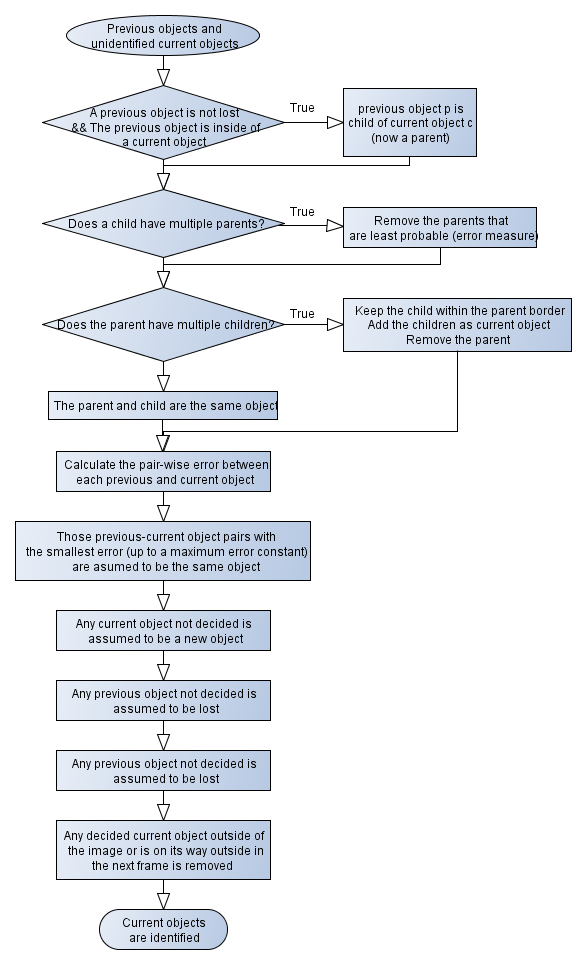
\includegraphics[width=123.5mm]{images/data_flow_identification.png}
	\caption{\textit{Flow chart of the 'Ultimate' algorithm. Each rectangular box may contain additional branches and loops leaving this figure to provide the reader with a overview of the occlusion handling progress and identification.}}
	\label{fig:ObjID_fig} %Skapar referens till figuren
\end{figure}
